

\documentclass{article}
\usepackage[utf8]{inputenc}
\usepackage[english]{babel}
\usepackage[]{amsthm} %lets us use \begin{proof}
\usepackage[]{amssymb} %gives us the character \varnothing
\usepackage{graphicx}
\usepackage{hyperref}
\usepackage{multicol}


\title{Homework 3}
\author{Aasim Zahoor}
\date\today


\begin{document}
\maketitle 


\begin{center}
\section{Problems}
\end{center}
\textbf{Link}\vspace{1.5em}
\url{https://github.com/AasimZahoor/Comp_methods.git}
\vspace{1.5em}

\textbf{Problem 1}\vspace{1.5em}
\\
In this problem I use two random matrices to test my matrix class. I used numpy's functionality to test some of the instances of the class. There were 7 instances in my class. So I tested addition, multiplication, transpose, trace, Determinant, Inverse and LU decomposition. The output is:
\\*
\\*
\begin{center}
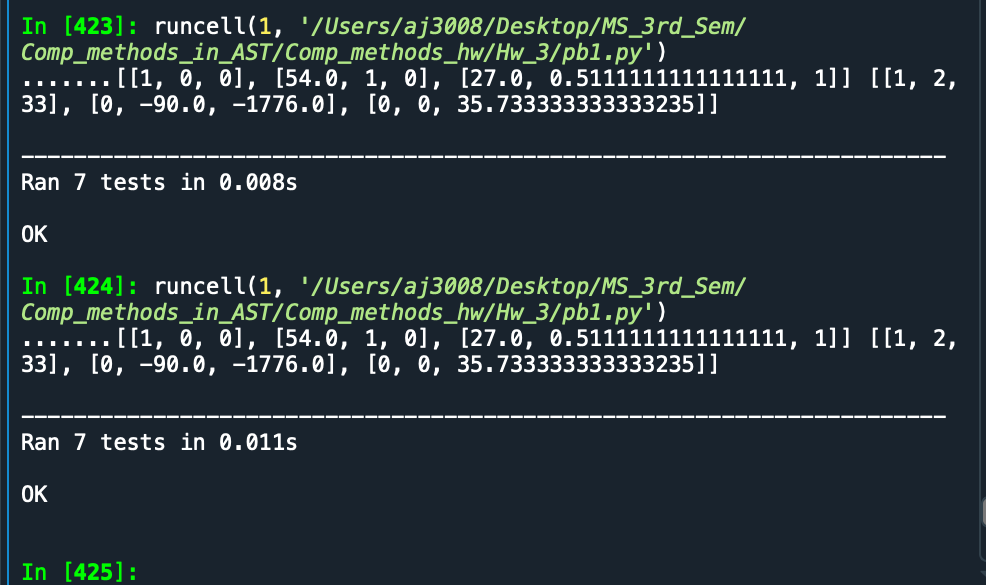
\includegraphics[scale=0.5]{/Users/aj3008/Desktop/MS_3rd_Sem/Comp_methods_in_AST/Comp_methods/Hw_3/Images/pb1}
\end{center}

\clearpage

\textbf{Problem 3}\vspace{1.5em}
\\
In the code for Problem 3 I have defined 3 functions. They are:
\begin{itemize}
\item{\textbf{euler$(x_0,y_0,f,h,k)$}}
This function call euler method for solving ODE. The arguments are:
\\*
       $ x_0$=initial x value
        $y_0$=initial y value
        $f$=function of x,y,t
        h=step size
        k=number of times
       \\*
        It returns x,y,t values in that order


\item{\textbf{heun$(x_0,y_0,f,h,k,p=10)$}}\vspace{0.2em}

This function call Heun's method for solving ODE. The arguments are:
\\*
        $x_0$=initial x value, 
        $y_0$=initial y value, 
        $f$=function of x,y,t, 
        h=step size, 
        k=number of times, 
        p=picard's iteration (Default value 10)
        \\*
        It returns x,y,t values in that order


\item{\textbf{rk$(x_0,y_0,f,h,k)$}}\vspace{0.2em}

This function call RK-4 method for solving ODE. The arguments are:
\\*
      $ x_0$=initial x value, 
        $y_0$=initial y value, 
        $f$=function of x,y,t, 
        h=step size, 
        k=number of times
        \\*
        It returns x,y,t values in that order


\vspace{0.2em}

\end{itemize}

\vspace{1.5em}
\textbf{Problem 4}\vspace{1.5em}
\\
In this problem we are supposed to test the functions we wrote in problem 3 using the pendulum function. To model the function I have made a function called \textbf{f(b,c)}. This function takes two arguments, b= coefficient of y, c= coefficient of g(x,t). This function returns an array where the first element gives d(theta)/dt and the second element returns d(omega)/dt. They values of b is taken as 0.25 and c as 5, step size is 0.1 and k (number of times) is 50 (to see the difference between the three methods) and 200 (to see how damping works).
\\



 \begin{center}
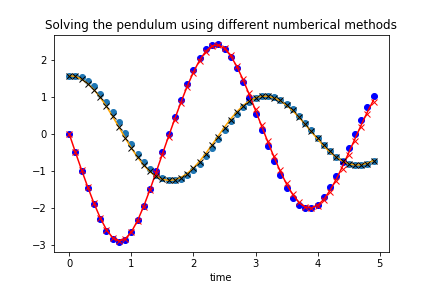
\includegraphics[scale=0.35]{/Users/aj3008/Desktop/MS_3rd_Sem/Comp_methods_in_AST/Comp_methods/Hw_3/Images/pb4}
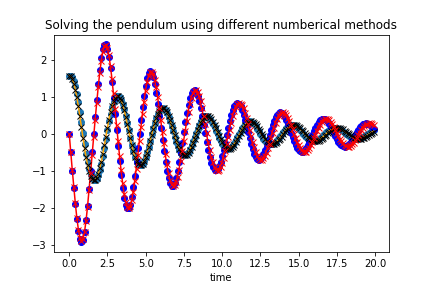
\includegraphics[scale=0.35]{/Users/aj3008/Desktop/MS_3rd_Sem/Comp_methods_in_AST/Comp_methods/Hw_3/Images/pb4_1}

\textbf{Figure}: The figure on the left is for k=50 and one on the right is for k=200
\end{center}

\vspace{0.2em}

\clearpage
\textbf{Problem 5}\vspace{1.5em}
\\
In this problem we are supposed to test our methods on the given equation. I defined a function \textbf{f(l)} which returns the function given in pb5. It takes lambda as input and gives an array as out where first element is always 1 and second element gives dy/dt in terms of y and t. The reason it gives 1 as the first element is because my ODE solvers were made for 2 dependent variables and this has only 1.


 \begin{center}
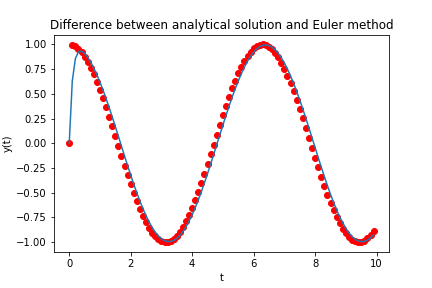
\includegraphics[scale=0.35]{/Users/aj3008/Desktop/MS_3rd_Sem/Comp_methods_in_AST/Comp_methods/Hw_3/Images/pb5_e}
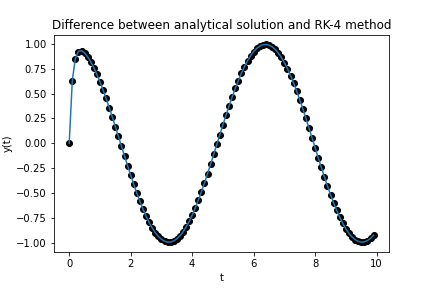
\includegraphics[scale=0.35]{/Users/aj3008/Desktop/MS_3rd_Sem/Comp_methods_in_AST/Comp_methods/Hw_3/Images/pb5_r}
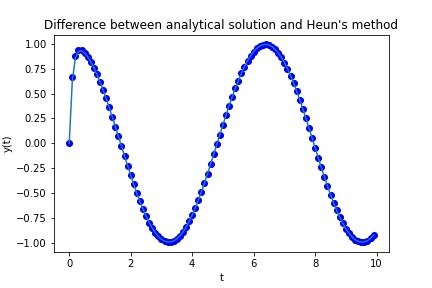
\includegraphics[scale=0.35]{/Users/aj3008/Desktop/MS_3rd_Sem/Comp_methods_in_AST/Comp_methods/Hw_3/Images/pb5_h}

\textbf{Figure}: These figures shows the three methods against the analytical solution.
\end{center}


        
     














\end{center}

\vspace{0.2em}
\end{document}
